% Copyright 2007-2010 Konrad-Zuse-Zentrum f�r Informationstechnik Berlin

% Licensed under the Apache License, Version 2.0 (the "License");
% you may not use this file except in compliance with the License.
% You may obtain a copy of the License at
%
%     http://www.apache.org/licenses/LICENSE-2.0
%
% Unless required by applicable law or agreed to in writing, software
% distributed under the License is distributed on an "AS IS" BASIS,
% WITHOUT WARRANTIES OR CONDITIONS OF ANY KIND, either express or implied.
% See the License for the specific language governing permissions and
% limitations under the License.
\documentclass[a4]{scrreprt}
\usepackage{typearea}
\areaset[1cm]{165mm}{240mm}

\usepackage[OT1]{fontenc}
\usepackage[latin1]{inputenc}

\usepackage{relsize}
\usepackage{graphicx}
%\usepackage{color}
%\usepackage{colortbl}
\usepackage{longtable}
\usepackage{makeidx}
\usepackage{ifthen}
\usepackage{fancyhdr}
\usepackage{fancyvrb}
\usepackage{lastpage}
\usepackage{xcolor}
\usepackage[pdftex,
        colorlinks=true,
        urlcolor=rltblue,       % \href{...}{...} external (URL)
        filecolor=rltblue,     % \href{...} local file
        linkcolor=rltblue,      % \ref{...} and \pageref{...}
%        pagebackref=true,
        pdfborder={0 0 0}]{hyperref}
\usepackage{listings}

\renewcommand{\headrulewidth}{0pt}    % Width of head rule
\renewcommand{\footrulewidth}{0.3pt}  % Width of head rule

% normal pages
\pagestyle{fancy}
\fancyhf{} % clear all header and footer fields
%\fancyhead[RE,LO]{}
\fancyhead[RO]{}%
\fancyfoot[LE,RO]{\bfseries\thepage\ / \pageref{LastPage}}%
\chead{}%
\cfoot{}%

% beginning of a chapter
\fancypagestyle{plain}{%
\fancyhf{} % clear all header and footer fields
%\fancyhead[RE,LO]{}
\fancyhead[RO]{}%
\fancyfoot[LE,RO]{\bfseries\thepage\ / \pageref{LastPage}}%
\chead{}%
\cfoot{}%
}

% Clear Header Style on the Last Empty Odd pages
\makeatletter
\def\cleardoublepage{\clearpage\if@twoside \ifodd\c@page\else%
    \hbox{}%
    \thispagestyle{empty}%              % Empty header styles
    \newpage%
    \if@twocolumn\hbox{}\newpage\fi\fi\fi}
\makeatother

%% Bold typewriter font
%\renewcommand{\ttdefault}{pcr}
%\renewcommand{\rmdefault}{ptm} % Times
%\renewcommand{\rmdefault}{ppl} % Palatino
%%\renewcommand{\rmdefault}{pnc} % NewCenturySchoolbook
%%\renewcommand{\rmdefault}{pbk} % BookMan
%\renewcommand{\rmdefault}{pag} % Avantgarde (sans serif)
%% \renewcommand{\rmdefault}{pzc} % ZapfChancery (slanted)
%\renewcommand{\rmdefault}{put} % Utopia
\renewcommand{\rmdefault}{bch} % CharterBT


%%% colors %%%%%%%%%%%%%%%%%%%%%%%%

\definecolor{lightyellow}{rgb}{1.0, 1.0, 0.5}
\definecolor{rltred}{rgb}{0.75,0,0}
\definecolor{rltgreen}{rgb}{0,0.5,0}


%\definecolor{rltblue}{rgb}{0,0,0.75}
\definecolor{rltblue}{HTML}{1F4980}
\definecolor{lightgray}{gray}{0.9}

\setlength{\parindent}{0pt}

% 31 73 128 blue

\definecolor{lightyellow}{rgb}{1.0, 1.0, 0.5}
\definecolor{codebackground}{rgb}{0.9,0.95,1.0}
\definecolor{commandinput}{rgb}{0.8,0.8,1}

%\thicklines
\lstset{
  basicstyle=\scriptsize\ttfamily,
  backgroundcolor=\color{codebackground},
  keywordstyle=\color{blue}\bfseries,
  % underlined bold black keywords
  identifierstyle=\bfseries, % nothing happens
  commentstyle=\color{red}\bfseries, % white comments
  stringstyle=\sffamily, % typewriter type for strings
  showstringspaces=false,
  xleftmargin=3pt,
  xrightmargin=3pt,
  fancyvrb=true,
  frame=single,
%  frameround=tttt,
%  framexleftmargin=0pt,
  framextopmargin=3pt,
  framexbottommargin=3pt,
%  framexrightmargin=5pt,
  rulecolor=\color{codebackground},
  language=Erlang,
%  fillcolor=\color{red},
%  rulesepcolor=\color{black}
%  rulesep=1cm,
}
\lstset{rangebeginprefix=\%\%\ userdevguide-begin\ }
\lstset{rangeendprefix=\%\%\ userdevguide-end\ }
\lstset{includerangemarker=false}

% \codesnippet[lstsettings]{filename-label}{range-label}{src-file with path}
% \codesnippet[language=Erlang]{admin.erl}{admin:add_nodes}{../src/admin.erl}
\newcommand{\codesnippet}[4][language=Erlang]{
{%% File: \url{#4}
\lstset{numbers=left}
\lstinputlisting[
  title=\filetitle{#2},
  linerange=#3-#3,
  #1
]
{#4}
}
}

% \codesfile[lstsettings]{filename-label}{src-file with path}
% \codesfile[language=Erlang]{admin.erl}{../src/admin.erl}
\newcommand{\codefile}[3][language=Erlang]{
{
\lstinputlisting[
  title=\filetitle{#2},
  #1]
{#3}
}
}
\newcommand\bfref[1]{\textbf{\hyperpage{#1}}}
\newcommand{\sieheref}[1]{\ref{#1} on page~\pageref{#1}}
\newcommand{\code}[1]{\lstinline[basicstyle=\small\ttfamily]!#1!}
\newcommand{\filetitle}[1]{\hbox to \linewidth{~~File \code{#1:}\hfill}}
\newcommand{\scalaris}{Scalaris}
\newcommand{\todo}[1]{{\color{red}{\em TODO: #1}}}
\newcommand{\svnrev}[1]
{\hfill\emph{Description is based on SVN revision #1.}\medskip}

\newcommand{\erlparamsorarity}[1]{%
\ifthenelse{\equal{/0}{#1}}{\texttt{#1}}{%
\ifthenelse{\equal{/1}{#1}}{\texttt{#1}}{%
\ifthenelse{\equal{/2}{#1}}{\texttt{#1}}{%
\ifthenelse{\equal{/3}{#1}}{\texttt{#1}}{%
\ifthenelse{\equal{/4}{#1}}{\texttt{#1}}{%
\ifthenelse{\equal{/5}{#1}}{\texttt{#1}}{%
\ifthenelse{\equal{/6}{#1}}{\texttt{#1}}{%
\ifthenelse{\equal{/7}{#1}}{\texttt{#1}}{%
\ifthenelse{\equal{/8}{#1}}{\texttt{#1}}{%
\ifthenelse{\equal{/9}{#1}}{\texttt{#1}}{%
(\texttt{#1})
}}}}}}}}}}}
\newcommand{\erlfun}[4][index]{%
\ifthenelse{\equal{index}{#1}}%
{\index{#2@\texttt{#2}!#3@\texttt{#3}}}%
{}%
\texttt{#2}:\-\texttt{#3}\erlparamsorarity{#4}}

\newcommand{\erlfunindex}[2]{%
\index{#1@\texttt{#1}!#2@\texttt{#2}|bfref}}%

\newcommand{\erlmodule}[2][index]{%
\ifthenelse{\equal{index}{#1}}%
{\index{#2@\texttt{#2}}}{}%
\texttt{#2}}

\newcommand{\erlmoduleindex}[1]{%
\index{#1@\texttt{#1}|bfref}}%

\makeatletter
\newenvironment{erlfunparams}
{
\list{}{
    \labelwidth\z@ \makeatother \itemindent-\leftmargin
    \let\makelabel\descriptionlabel
\setlength\leftmargin{4em}
\setlength{\parskip}{0pt}
\setlength{\parsep}{0pt}
\setlength{\itemsep}{0pt}
}}
{\endlist}
\makeatother
\newcommand{\erlparam}[2]{\item[\texttt{#1}:] #2}

\newenvironment{wikitext}
{\catcode`\#=13\catcode`\$=13\catcode`\_=11\catcode`\==13
}{\catcode`\#=6\catcode`\$=3\catcode`\_=8}


\makeindex

\begin{document}
\vspace*{4cm}
\thispagestyle{empty}
\setlength{\parskip}{1ex}
\begin{tabular}{p{4cm}p{0.5cm}p{10cm}}
%\vspace*{-5cm}
\includegraphics[width=5cm]{scalaris-layers}
\parbox{4cm}{
\includegraphics[width=4cm]{scalaris-layers}}
& &\sffamily\bfseries\Huge
  \bigskip {\textcolor{rltblue}{Scalaris:}}

\medskip
 \mdseries Users and Developers Guide

\bigskip\medskip
\LARGE Version 0.2.0 draft \hfill \today\\
\end{tabular}
\vfill
{\scriptsize
Copyright 2007-2010 Konrad-Zuse-Zentrum f�r Informationstechnik Berlin
and onScale solutions.

Licensed under the Apache License, Version 2.0 (the "License");
you may not use this file except in compliance with the License.
You may obtain a copy of the License at

\url{http://www.apache.org/licenses/LICENSE-2.0}

Unless required by applicable law or agreed to in writing, software
distributed under the License is distributed on an "AS IS" BASIS,
WITHOUT WARRANTIES OR CONDITIONS OF ANY KIND, either express or implied.
See the License for the specific language governing permissions and
limitations under the License.
}

\tableofcontents

\part{Users Guide}

\chapter{Introduction}

Scalaris is a scalable, transactional, distributed key-value store based on
the peer-to-peer principle. It can be used to build scalable Web 2.0
services. The concept of Scalaris is quite simple: Its architecture consists
of three layers.

It provides self-management and scalability by replicating services and data
among peers. Without system interruption it scales from a few PCs to
thousands of servers. Servers can be added or removed on the fly without any
service downtime.

\begin{center}
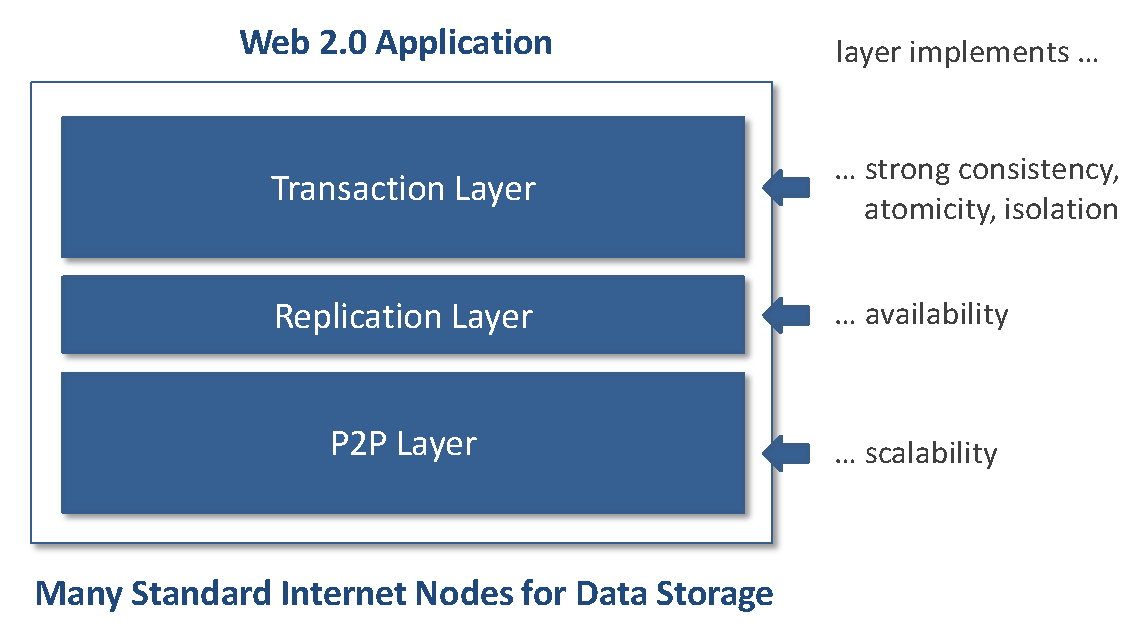
\includegraphics[width=0.7\linewidth]{layers}
\end{center}

Scalaris takes care of:

\begin{itemize}
\item Fail-over
\item Data distribution
\item Replication
\item Strong consistency
\item Transactions
\end{itemize}

The Scalaris project was initiated by Zuse Institute Berlin and onScale
solutions and was partly funded by the EU projects Selfman and
XtreemOS. Additional information (papers, videos) can be found at
\url{http://www.zib.de/CSR/Projects/scalaris} and
\url{http://www.onscale.de/scalarix.html}.

\section{Brewer's CAP Theorem}

In distributed computing there exist the so called CAP theorem. It
basically says that in distributed systems there are three desirable
properties for such systems but can have only any two of them.

\begin{description}
\item {Strict Consistency.} Any read operation has to return the
  result of the latest write operation on the same data item.

\item {Availability.} Items can be read and modified at any time.

\item {Partition Tolerance.} The network on which the service is
  running may split into several partitions which cannot communicate
  with each other. Lateron the may rejoin again.

  For example, a service is hosted on one machine in Seattle and one
  machine in Berlin. This service is partition tolerant if it can
  tolerate that all Internet connections over the Atlantic (and
  Pacific) are interrupted for a few hours and then get repaired
  afterwards.
\end{description}

The goal of \scalaris{} is to provide strict consistency and partition
tolerance. We are willing to sacrifice availability to make sure that
the stored data is always consistent. I.e. when you are running
\scalaris{} with a replication degree of 4 and the network splits into
two partitions, one partition with three replicas and one partition
with one replica, you will be able to continue to use the service only
in the larger partition. All requests in the smaller partition will
time out until the two networks merge again. Note, most other
key-value stores tend to sacrifice consistency.

\chapter{Download and Installation}

\section{Requirements}

For building and running \scalaris{}, some third-party modules are
required which are not included in the \scalaris{} sources:

\begin{itemize}
\setlength{\itemsep}{0pt}
\setlength{\parskip}{0pt}
\item Erlang R12 or newer
\item GNU-like Make
\end{itemize}

Note, the Version 13 of Erlang is required. \scalaris{} will not
work with older versions.

To build the Java API (and the command-line client) the following
modules are required additionally:

\begin{itemize}
\setlength{\itemsep}{0pt}
\setlength{\parskip}{0pt}
\item Java Development Kit 1.6
\item Apache Ant
\end{itemize}

Before building the Java API, make sure that \code{JAVA\_HOME} and
\code{ANT\_HOME} are set. \code{JAVA\_HOME} has to point to a JDK
1.6 installation, and \code{ANT\_HOME} has to point to an Ant
installation.

\section{Download}

The sources can be obtained from
\url{http://code.google.com/p/scalaris}. RPMs are available from
\url{http://download.opensuse.org/repositories/home:/tschuett/}.

\subsection{Development Branch}

You find the latest development version in the svn repository:
\begin{lstlisting}[language=sh]
# Non-members may check out a read-only working copy anonymously over HTTP.
svn checkout http://scalaris.googlecode.com/svn/trunk/ scalaris-read-only
\end{lstlisting}

\subsection{Releases}

Releases can be found under the 'Download' tab on the web-page.


\section{Configuration}

\scalaris{} reads two configuration files from the working directory:
\code{bin/scalaris.cfg} (mandatory) and \code{bin/scalaris.local.cfg}
(optional). The former defines default settings and is included in the
release. The latter can be created by the user to alter settings.  A
sample file is \code{bin/scalaris.local.cfg.example}. To run \scalaris{}
distributed over several nodes, each node requires a \code{bin/scalaris.local.cfg}:

\codefile{scalaris.local.cfg}{../bin/scalaris.local.cfg.example}

\scalaris{} distinguishes currently two different kinds of nodes: (a)
the boot-server and (b) regular nodes. For the moment, we limit the
number of boot-servers to exactly one. The remaining nodes are regular
nodes. The boot-server is contacted to join the system. On all servers,
the \code{boot_host} option defines the server where the boot server
is running. In the example, it is an IP address plus a TCP port.

\section{Build}

\subsection{Linux}

\scalaris{} uses autoconf for configuring the build environment and
GNU Make for building the code.

\begin{lstlisting}[language=sh]
%> ./configure
%> make
%> make docs
\end{lstlisting}

For more details read \code{README} in the main \scalaris{} checkout
directory.

\subsection{Windows}

We are currently not supporting \scalaris{} on Windows. However, we
have two small {\tt bat} files for building and running a boot
server. It seems to work but we make no guarantees.

For the most recent description please see the FAQ at
\url{http://code.google.com/p/scalaris/wiki/FAQ}.

% \begin{itemize}
% \item Install Erlang
% \item Install OpenSSL (for crypto module)
% \item Checkout scalaris code from SVN
% \item copy an appropriate EMakefile\_for from \code{contrib/win32} to the trunk-directory
% \item Adapt the path to your Erlang installation in build.bat
% \item run build.bat
% \item Go to the bin sub-directory
% \item Adapt the path to your Erlang installation in boot.bat
% \item run boot.bat
% \end{itemize}

\subsection{Java-API}

The following commands will build the Java API for \scalaris{}:
\begin{lstlisting}[language=sh]
%> make java
\end{lstlisting}

This will build scalaris.jar, which is the library for accessing
the overlay network. Optionally, the documentation can be build:
\begin{lstlisting}[language=sh]
%> cd java-api
%> ant doc
\end{lstlisting}


\section{Running \scalaris{}}

As mentioned above, in \scalaris{} there are two kinds of nodes:
\begin{itemize}
\setlength{\itemsep}{0pt}
\setlength{\parskip}{0pt}
\item boot servers
\item regular nodes
\end{itemize}

In every \scalaris{}, at least one boot server is required. It will
maintain a list of nodes taken part in the system and allows other
nodes to join the ring. For redundancy, it is also possible to have
several boot servers. In the future, we want to eliminate this
distinction, so any node is also a boot-server.

\subsection{Running on a local machine}
\label{sec.boot}

Open at least two shells. In the first, go into the bin directory:
\begin{lstlisting}[language=sh]
%> cd bin
%> ./boot.sh
\end{lstlisting}

This will start the boot server. On success \url{http://localhost:8000}
should point to the management interface page of the boot server. The main
page will show you the number of nodes currently in the system. After a
couple of seconds a first \scalaris{} should have started in the boot server
and the number should increase to one. The main page will also allow you to
store and retrieve key-value pairs.

%The boot server should show output similar to the following, when
%starting the first \scalaris{} nodes. The first line is printed when
%the \scalaris{} is spawned. Afterwards it will try to connect the
%boot server. When the third line is printed, it managed to contact the
%boot server and joined the ring. In this case, it was the first node
%in the ring.
%\begin{lstlisting}
%[ I | Node   | <0.97.0> ] joining "23947834870"
%[ I | Node   | <0.97.0> ] join as first [50,51,57,52,55,56,51,52,56,55,48]
%[ I | Node   | <0.97.0> ] joined
%\end{lstlisting}

In a second shell, you can now start a second \scalaris{} node. This
will be a `regular server'. Go in the bin directory:
\begin{lstlisting}[language=sh]
%> cd bin
%> ./cs_local.sh
\end{lstlisting}

The second node will read the configuration file and use this
information to contact the boot server and will join the ring. The
number of nodes on the web page should have increased to two by now.

Optionally, a third and fourth node can be started on the same
machine. In a third shell:
\begin{lstlisting}[language=sh]
%> cd bin
%> ./cs_local2.sh
\end{lstlisting}


In a fourth shell:
\begin{lstlisting}[language=sh]
%> cd bin
%> ./cs_local3.sh
\end{lstlisting}


This will add 3 nodes to the network. The web pages at
\url{http://localhost:8000} should show the additional nodes.

\subsection{Running distributed}

\scalaris{} can be installed on other machines in the same way as
described in Sect.~\ref{sec:install}. In the default configuration,
nodes will look for the boot server on localhost on port 14195. You
should create a \code{scalaris.local.cfg} pointing to the node running
the boot server.

\begin{lstlisting}[language=Erlang]
% Insert the appropriate IP-addresses for your setup
% as comma separated integers:
% IP Address, Port, and label of the boot server
{boot_host, {{127,0,0,1},14195,boot}}.
\end{lstlisting}

If you are using the default configuration on the boot server it will
listen on port 14195 and you only have to change the IP address in the
configuration file. Otherwise the other nodes will not find the boot
server. On the remote nodes, you only need to call
\code{./cs_local.sh} and they will automatically contact the
configured boot server.

%\subsection{Running on PlanetLab}

%\subsection{Replication Degree}

%\subsection{Routing Scheme}

\section{Installation}
\label{sec:install}

For simple tests, you do not need to install \scalaris{}. You can run
it directly from the source directory. Note: \code{make install} will
install scalaris into \code{/usr/local}. But is more convenient to
build RPMs and install those.

\begin{lstlisting}{language=sh}
svn checkout http://scalaris.googlecode.com/svn/trunk/ scalaris-0.0.1
tar -cvjf scalaris-0.0.1.tar.bz2 scalaris-0.0.1 --exclude-vcs
cp scalaris-0.0.1.tar.bz2 /usr/src/packages/SOURCES/
rpmbuild -ba scalaris-0.0.1/contrib/scalaris.spec
\end{lstlisting}

Your source and binary rpm will be generated in
/usr/src/packages/SRPMS and RPMS.  We also build rpms using checkouts
from svn and provide them using the openSUSE BuildService at
http://download.opensuse.org/repositories/home:/tschuett/. RPM
packages are available for

\begin{itemize}
\item Fedora 9, 10,
\item Mandriva 2008, 2009,
\item openSUSE 11.0, 11.1,
\item SLE 10, 11,
\item CentOS 5 and
\item RHEL 5.
\end{itemize}

Inside those repositories you will also find an erlang rpm - you don't
need this if you already have a recent enough erlang version!

\section{Logging}
\label{sec:logging}

\scalaris{} uses the log4erl library (see \code{contrib/log4erl} for
logging status information and error messages. The log level can be
configured in \code{bin/scalaris.cfg}.  The default value is {\tt
  error}; only errors and severe problems are logged.

\begin{lstlisting}[language=Erlang]
%% @doc Loglevel: debug < info < warn < error < fatal < none
{log_level, error}.
\end{lstlisting}

In some cases, it might be necessary to get more complete logging
information, e.g. for debugging. In \sieheref{sec:start-addit-local},
we are explaining the startup process of \scalaris{} nodes in more
detail, here the {\tt info} level provides more detailed information.

\begin{lstlisting}[language=Erlang]
%% @doc Loglevel: debug < info < warn < error < fatal < none
{log_level, info}.
\end{lstlisting}

\chapter{Using the system}

\section{JSON API}

\scalaris{} supports a JSON API for transactions. To minimize the necessary
round trips between a client and \scalaris{}, it uses request lists, which
contain all requests that can be done in parallel. The request list is then
send over to a \scalaris{} node with a POST message. The result is an opaque
TransLog and a list containing the results of the requests. To add further
requests to the transaction, the TransLog and another list of requests may
be send to \scalaris{}.  This process may be repeated as necessary. To finish
the transaction, the request list can contain a 'commit' request as last
element, which triggers the validation phase of the transaction processing.

The JSON-API can be accessed via the \scalaris{}-Web-Server running on port
8000 by default and the page \code{jsonrpc.yaws} (For example at:
\url{http://localhost:8000/jsonrpc.yaws}).  The following example
illustrates the message flow:

\begin{longtable}{p{0.45\textwidth}cp{0.45\textwidth}}
\bf Client & & \bf \scalaris{} node \\
Make a transaction, that sets two keys:
\begin{lstlisting}[language=java]
{
  "method":"req_list",
  "version":"1.1",
  "params":
    [
      [
        { "write":{"keyA":"valueA"} },
        { "write":{"keyB":"valueB"} },
        { "commit":"commit" }
      ]
    ],
  "id":0
}
\end{lstlisting}
& $\to$
& \\

& $\leftarrow$ &
\scalaris{} sends results back
\begin{lstlisting}[language=java]
{ "result":
  { "results":
      [
        { "op":"commit",
          "value":"ok",
          "key":"ok" },
        { "op":"write",
          "value":"valueB",
          "key":"keyB" },
        { "op":"write",
          "value":"valueA",
          "key":"keyA" }
      ],
    "translog":
     [...]
  },
  "id" : 0
}
\end{lstlisting}
\\

In a second transaction: Read the two keys
\begin{lstlisting}[language=java]
{
  "method":"req_list",
  "version":"1.1",
  "params":
    [
      [
        { "read":"keyA" },
        { "read":"keyB" }
      ]
    ]
  "id":0
}
\end{lstlisting}
& $\to$ & \\

& $\leftarrow$ &
\scalaris{} sends results back
\begin{lstlisting}[language=java]
{ "result":
  {"results":
    [
      { "op":"read",
        "value":"valueB",
        "key":"keyB" },
      { "op":"read",
        "value":"valueA",
        "key":"keyA" }
    ],
   "translog":
    [...] // this list is the translog
          // for further operations!
          // We name it TLOG here.
  },
  "id" : 0
}
\end{lstlisting}\\

Calculate something with the read values and make further requests, here a
write and the commit for the whole transaction. Include also the latest
translog we got from \scalaris{} (named \code{TLOG} here).

\begin{lstlisting}[language=java]
{
  "method":"req_list",
  "version":"1.1",
  "params":
    [
      TLOG, // translog from prev. result.
      [
        { "write":{"keyA":"valueA2"} },
        { "commit":"commit" }
      ]
    ],
  "id" : 0
}
\end{lstlisting}
& $\to$ & \\

& $\leftarrow$ &
\scalaris{} sends results back
\begin{lstlisting}[language=java]
{ "result":
  { "results":
    [ { "op":"commit",
        "value":"ok",
        "key":"ok" },
      { "op":"write",
        "value":"valueA2",
        "key":"keyA" }
    ],
    "translog":
    [...]
  },
  "id" : 0
}
\end{lstlisting}\\
\end{longtable}

A sample usage of the JSON API using Ruby can be found in \code{contrib/jsonrpc.rb}.

A single request list must not contain a key more than once!

The allowed requests are:
\begin{lstlisting}[language=java]
{ "read":"any_key" }

{ "write":{"any_key":"any_value"} }

{ "commit":"commit" }
\end{lstlisting}

The possible results are:
\begin{lstlisting}[language=java]
{ "op":"read", "key":"any_key", "value":"any_value" }
{ "op":"read", "key":"any_value", "fail":"reason" } // 'not_found' or 'timeout'

{ "op":"write",  "key":"any_key", "value":"any_value" }
{ "op":"read", "key":"any_key", "fail":"reason" }

{ "op":"commit", "value":"ok", "key":"ok" }
{ "op":"commit", "value":"fail", "fail":"reason" }
\end{lstlisting}

\subsection{Deleting a key}

Outside transactions keys can also be deleted, but it has to be done with
care, as explained in the following thread on the mailing list:
\url{http://groups.google.com/group/scalaris/browse_thread/thread/ff1d9237e218799}.

\begin{lstlisting}[language=java]
{
  "method":"delete",
  "version":"1.1",
  "params":
    [
      { "key":"any_key" }
    ],
  "id" : 0
}
\end{lstlisting}

Two sample results

\begin{lstlisting}[language=java]
{ "result":
  { "ok":2, // how many replicas were deleted successsfully
    "results": [ "ok", "ok", "locks_set", "undef" ]
  }
}
\end{lstlisting}

\begin{lstlisting}[language=java]
{ "result":
  { "failure":"reason" }
}
\end{lstlisting}


%\section{Erlang}

\section{Java command line interface}

The jar file contains a small command line interface client. For
convenience, we provide a wrapper script called \code{scalaris} which
setups the Java environment:

\begin{lstlisting}[language=sh]
%> cd java-api
%> ./scalaris -help
usage: scalaris
 -g,--getsubscribers <topic>   get subscribers of a topic
 -help                         print this message
 -minibench                    run mini benchmark
 -p,--publish <params>         publish a new message for a topic: <topic>
                               <message>
 -r,--read <key>               read an item
 -s,--subscribe <params>       subscribe to a topic: <topic> <url>
 -u,--unsubscribe <params>     unsubscribe from a topic: <topic> <url>
 -w,--write <params>           write an item: <key> <value>
\end{lstlisting}

Read and write can be used to read resp. write from/to the
overlay. getsubscribers, publish, and subscribe are the PubSub
functions.

\begin{lstlisting}[language=sh]
%> ./scalaris -write foo bar
write(foo, bar)
%> ./scalaris -read foo
read(foo) == bar
\end{lstlisting}

The scalaris library requires that you are running a `regular server' on
the same node. Having a boot server running on the same node is not
sufficient.

\section{Java API}

The \code{scalaris.jar} provides the command line client as well as a
library for Java programs to access \scalaris{}. The library provides two classes:

\begin{itemize}
\item \code{Scalaris} provides a high-level API similar to the command line client.
\item \code{Transaction} provides a low-level API to the transaction
  mechanism.
\end{itemize}

For details we refer the reader to the Javadoc:

\begin{lstlisting}[language=sh]
%> cd java-api
%> ant doc
%> firefox doc/index.html
\end{lstlisting}

\chapter{Testing the system}

\section{Running the unit tests}
There are some unit tests in the \code{test} directory. You can call them
by running \code{make test} in the main directory. The results are stored
in a local \code{index.html} file. 

The tests are implemented with the \code{common-test} package from the
Erlang system. For running the tests we rely on \code{run\_test},
which is part of the \code{common-test} package, but is not installed
by default. \code{configure} will check whether \code{run\_test} is
available. If it is not installed, it will show a warning and a short
description of how to install the missing file.

Note: for the unit tests, we are setting up and shutting down several
overlay networks. During the shut down phase, the runtime environment
will print extensive error messages. These error messages do not
indicate that tests failed! Running the complete test suite takes
about 5 minutes. Only when the complete suite finished, it will
present statistics on failed and successful tests.

\chapter{Troubleshooting}

\section{Network}

\scalaris{} uses a couple of TCP ports for communication. It does
not use UDP at the moment.

\begin{tabular}{ll}
8000 & HTTP Server on the boot node\\
8001 & HTTP Server on the other nodes\\
14195 & Port for inter-node communication (boot server)\\
14196 & Port for inter-node communication (other nodes)\\
\end{tabular}

Please make sure that at least 14195 and 14196 are not blocked by
firewalls.


\part{Developers Guide}

\chapter{General Hints}

\section{Coding Guidelines}

\begin{itemize}
\item Keep the code short
\item Use \erlmodule{gen\_component} to implement additional processes
\item Don't use receive by yourself (Exception: to implement single threaded
  user API calls (cs\_api, yaws\_calls, etc)
\item Don't use \erlfun{erlang}{now}{}, \erlfun{erlang}{send\_after}{},
  \erlmodule{receive after} etc. in performance critical code, consider
  using \erlmodule{msg\_delay} instead.
\item Don't use \erlfun{tc}{timer}{} as it catches exceptions
\end{itemize}

\section{Testing Your Modifications and Extensions}

\begin{itemize}
\item Run the testsuites using make test
\item Run the java api test using make java-test
      (or if you want to see the scalaris output during the tests, start a
      bin/boot.sh and run the tests by cd java; ant test)
\item Run the Ruby client by starting Scalaris and running cd contrib; ./jsonrpc.rb
\end{itemize}

\section{Help with Digging into the System}
\label{sec:digging}

\begin{itemize}
\item use ets:i() to get details on the local state of some processes
\item consider changing pdb.erl to use ets instead of erlang:put/get
\item Have a look at strace -f -p PID of beam process
\item Get message statistics via the Web-interface
\item enable/disable tracing for certain modules
%% \item enable gen-component profiling and read the collected data using
%% 
%%    \code{lists:reverse(lists:keysort(2,ets:tab2list(profiling))).}
%% 
%%    (Has the limitation that it measures using absolute time, maybe the data
%%    is more ok, when using -smp disable? ...)
\item Use etop and look at the total memory size and atoms generated
\item send processes sleep or kill messages to test certain behaviour (see
  gen\_component.erl
\item use \code{boot_server:number_of_nodes(). flush().}
\item use \code{admin_checkring(). flush().}
\end{itemize}

\chapter{System Infrastructure}

\section{The Process Dictionary}
\label{sec:process_dictionary}
\erlmoduleindex{process\_dictionary}

\begin{itemize}
\item What is it? How to distinguish from Erlangs internal process dictionary?
\item Joining a process group (InstanceId id a group name)
\item Why we do this... (managing several independent nodes inside a single
  Erlang VM)
\end{itemize}

\section{The Communication Layer \erlmodule{comm}}
\label{sec:comm}
\erlmoduleindex{comm}

\begin{itemize}
\item in general
\item format of messages (tuples)
\item use messages with cookies (server and client side)
\item What is a message tag?
\end{itemize}

\section{\texorpdfstring{The \erlmodule{gen\_component}}
         {The gen\_component}}
\erlmoduleindex{gen\_component}
\svnrev{r2675}

The generic component model implemented by
\erlmodule[noindex]{gen\_component} allows to add some common functionality
to all the components that build up the \scalaris{} system. It supports:

\begin{description}
\setlength{\parskip}{0pt}
\setlength{\itemsep}{0pt}
\item[event-handlers:] message handling with a similar syntax as used in \cite{rachid-book}.
\item[FIFO order of messages:] components cannot be inadvertently locked as
  we do not use selective receive statements in the code.
\item[sleep and halt:] for testing components can sleep or be halted.
\item[debugging, breakpoints, stepwise execution:] to debug components
  execution can be steered via breakpoints, step-wise execution and
  continuation based on arriving events and user defined component state
  conditions.
\item[basic profiling,]
\item[state dependent message handlers:] depending on its state, different
  message handlers can be used and switched during runtime. Thereby a kind
  of state-machine based message handling is supported.
\item[prepared for \erlmodule{pid\_groups}:] allows to send events to
  named processes inside the same group as the actual component itself
  (\code{send_to_group_member}) when just holding a reference to any group
  member, and
\item[unit-testing of event-handlers:] as message handling is separated from
  the main loop of the component, the handling of individual messages and
  thereby performed state manipulation can easily tested in unit-tests by
  directly calling message handlers.
\end{description}

In \scalaris{} all Erlang processes should be implemented as
\erlmodule{gen\_component}. The only exception are functions interfacing to
the client, where a transition from asynchronous to synchronous request
handling is necessary and that are executed in the context of a client's
process or a process that behaves as a proxy for a client
(\erlmodule{cs\_api}).

\subsection{\texorpdfstring{A basic \erlmodule{gen\_component} including a message handler}
             {A basic gen\_component including a message handler}}

To implement a \erlmodule{gen\_component}, the component has to provide the
\erlmodule{gen\_component} behaviour:

\codesnippet{gen_component.erl}{gen_component:behaviour}{../src/gen_component.erl}

This is illustrated by the following example:

\codesnippet{msg_delay.erl}{gen_component:sample}{../src/msg_delay.erl}

\erlfun{your\_gen\_component}{init}{/1} is called during start-up of a
\erlmodule{gen\_component} and should return the initial state to be used
for this \erlmodule{gen\_component}. Later, the current state of the
component can be retrieved using \erlfun{gen\_component}{get\_state}{/1}.

To react on messages / events, a message handler is used. The default
message handler is given to or
\erlfun{gen\_component}{start\_link}{/4} as well as
\erlfun{gen\_component}{start}{/4} or
\erlfun{gen\_component}{start}{/5}. It can be
changed by calling \erlfun{gen\_component}{change\_handler}{/2} (see
Section~\ref{sec:gen_component:change_handler}). When an event / message for
the component arrives, this handler is called with the event itself and the
current state of the component. In the handler, the state of the component
may be adjusted depending upon the event. The handler itself may trigger new
events / messages for itself or other components and has finally to return
the updated state of the component or the atoms \texttt{unknown\_event} or
\texttt{kill}. It must neither call \code{receive} nor
\erlfun{timer}{sleep}{/1} nor \erlfun{erlang}{exit}{/1}.

\subsection{\texorpdfstring{How to start a \erlmodule{gen\_component}?}
             {How to start a gen\_component?}}

A \erlmodule{gen\_component} can be started using one of:

\erlfun{gen\_component}{start}{Module, Handler, Args, GenCOptions = []}\\
\erlfun{gen\_component}{start\_link}{Module, Handler, Args, GenCOptions = []}
\begin{erlfunparams}
\erlparam{Module}{the name of the module your component is
   implemented in}
   \erlparam{Handler}{the inital message handler}
\erlparam{Args}{List of parameters passed to \code{Module:init/1}
   for initialization}
\erlparam{GenCOptions}{optional parameter.
   List of options for \erlmodule{gen\_component}
\begin{description}
\setlength{\parskip}{0pt}
\setlength{\itemsep}{0pt}
\item[\texttt{\{pid\_groups\_join\_as, ProcessGroup, ProcessName\}}:] registers the new
  process with the given process group (also called instanceid) and name
  using \erlmodule{pid\_groups}.
\item[\texttt{\{erlang\_register, ProcessName\}}:] registers the process as
  a named Erlang process.
\item[\texttt{\{wait\_for\_init\}}:] wait for \code{Module:init/1} to return
  before returning to the caller.
\end{description}
}
\end{erlfunparams}

These functions are compatible to the Erlang/OTP supervisors.  They spawn a
new process for the component which itself calls \code{Module:init/1} with
the given \code{Args} to initialize the component. \code{Module:init/1}
should return the initial state for your component. For each message sent to
this component, the default message handler
\erlfun[noindex]{Module}{on}{Message, State} will be called, which should
react on the message and return the updated state of your component.

\erlfun{gen\_component}{start}{} and \erlfun{gen\_component}{start\_link}{}
return the pid of the spawned process as \code{\{ok, Pid\}}.


\subsection{\texorpdfstring{When does a \erlmodule{gen\_component} terminate?}
             {When does a gen\_component terminate?}}

A \erlmodule{gen\_component} can be stopped using:

\erlfun{gen\_component}{kill}{Pid} or by returning \code{kill} from the
current message handler.

\subsection{\texorpdfstring{How to determine whether a process is a \erlmodule{gen\_component}?}
             {How to determine whether a process is a gen\_component?}}

A \erlmodule{gen\_component} can be detected by:

\erlfun{gen\_component}{is\_gen\_component}{Pid}, which returns a boolean.

\subsection{What happens when unexpected events / messages arrive?}

Your message handler (default is \erlfun{your\_gen\_component}{on}{/2})
should return \code{unknown_event} in the final clause
(\erlfun{your\_gen\_component}{on}{\_,\_}).  \erlmodule{gen\_component} then
will nicely report on the unhandled message, the component's name, its state
and currently active message handler, as shown in the following example:

\begin{lstlisting}[language=bash]
# bin/boot.sh
[...]
(boot@localhost)10> pid_groups ! {no_message}.
{no_message}
[error] unknown message: {no_message} in Module: pid_groups and
handler on in State null
(boot@localhost)11>
\end{lstlisting}

The \erlmodule{pid\_groups} (see
Section~\ref{sec:pid_groups}) is a \erlmodule{gen\_component} which
registers itself as named Erlang process with the \erlmodule{gen\_component}
option \code{erlang_register} and therefore can be addressed by its name in
the Erlang shell. We send it a \code{\{no_message\}} and
\erlmodule{gen\_component} reports on the unhandled message. The
\erlmodule{pid\_groups} module itself continues to run and waits for
further messages.

\subsection{What if my message handler generates an exception or
 crashes the process?}

\erlmodule{gen\_component} catches exceptions generated by message handlers
and reports them with a stack trace, the message, that generated the
exception, and the current state of the component.

If a message handler terminates the process via \erlfun{erlang}{exit}{/1},
this is out of the responsibility scope of \erlmodule{gen\_component}. As
usual in Erlang, all linked processes will be informed. If for example
\erlfun{gen\_component}{start\_link}{/2} or \texttt{/3} was used for
starting the \erlmodule{gen\_component}, the spawning process will be
informed, which may be an Erlang supervisor process taking further actions.

\subsection{Changing message handlers and implementing state dependent
 message responsiveness as a state-machine}
\label{sec:gen_component:change_handler}
\erlfunindex{gen\_component}{change\_handler}

Sometimes it is beneficial to handle messages depending on the state of a
component. One possibility to express this is implementing different clauses
depending on the state variable, another is introducing case clauses inside
message handlers to distinguish between current states. Both approaches may
become tedious, error prone, and may result in confusing source code.

Sometimes the use of several different message handlers for different states
of the component leads to clearer arranged code, especially if the set of
handled messages changes from state to state. For example, if we have a
component with an initialization phase and a production phase afterwards, we
can handle in the first message handler messages relevant during the
initialization phase and simply queue all other requests for later
processing using a common default clause.

When initialization is done, we handle the queued user requests and switch
to the message handler for the production phase. The message handler for the
initialization phase does not need to know about messages occurring during
production phase and the message handler for the production phase does not
need to care about messages used during initialization. Both handlers can be
made independent and may be extended later on without any adjustments to the
other.

One can also use this scheme to implement complex state-machines by changing
the message handler from state to state.

To switch the message handler
\erlfun{gen\_component}{change\_handler}{State, new\_handler} is called as
the last operation after a message in the active message handler was
handled, so that the return value of
\erlfun{gen\_component}{change\_handler}{/2} is propagated to
\erlmodule{gen\_component}.  The new handler is given as an atom, which is
the name of the 2-ary function in your component module to be called.

\subsubsection{Starting with non-default message handler.}
It is also possible to change the message handler right from the start
in your \erlfun{your\_gen\_component}{init}{/1} to avoid the default message
handler \erlfun{your\_gen\_component}{on}{/2}. Just create your initial
state as usual and call \erlfun{gen\_component}{change\_handler}{State,
  my\_handler} as the final call in your
\erlfun{your\_gen\_component}{init}{/1}. We prepared
\erlfun{gen\_component}{change\_handler}{/2} to return \code{State} itself,
so this will work properly.

\subsection{Handling several messages atomically}

The message handler is called for each message separately. Such a single
call is atomic, i.e. the component does not perform any other action until
the called message handler finishes. Sometimes, it is necessary to execute
two or more calls to the message handler atomically (without other
interleaving messages). For example if a message \code{A} contains another
message \code{B} as payload, it may be necessary to handle \code{A} and
\code{B} directly one after the other without interference of other
messages. So, after handling \code{A} you want to call your message handler
with \code{B}.

In most cases, you could just do so by calculating the new state as result
of handling message \code{A} first and then calling the message handler with
message \code{B} and the new state by yourself.

It is safer to use \erlfun{gen\_component}{post\_op}{2} in such cases: When
$B$ contains a special message, which is usually handled by the
\erlmodule{gen\_component} module itself (like
\code{send\_to\_group\_member}, \code{kill}, \code{sleep}), the direct call
to the message handler would not achieve the expected result. By calling
\erlfun{gen\_component}{post\_op}{B, NewState} to return the new state after
handling message \code{A}, message \code{B} will be handled directly after
the current message \code{A}.

\subsection{\texorpdfstring{Halting and pausing a \erlmodule{gen\_component}}
{Halting and pausing a gen\_component}}

Using \erlfun{gen\_component}{kill}{Pid} and
\erlfun{gen\_component}{sleep}{Pid, Time} components can be terminated or
paused.

\subsection{\texorpdfstring{Integration with \erlmodule{pid\_groups}:
  Redirecting messages  to other \erlmodule{gen\_component}s}
  {Integration with pid\_groups:
  Redirecting messages  to other gen\_components}}

Each \erlmodule{gen\_component} by itself is prepared to support
\erlfun{comm}{send\_to\_group\_member}{/3} which forwards messages inside a
group of processes registered via \erlmodule{pid\_groups} (see
Section~\ref{sec:pid_groups}) by their name. So, if you hold a Pid
of one member of a process group, you can send messages to other members of
this group, if you know their registered Erlang name. You do not necessarily
have to know their individual Pid.

\emph{In consequence, no \erlmodule{gen\_component} can individually handle
  messages of the form \code{\{send_to_group_member,} \code{_, _\}} as such
  messages are consumed by \erlmodule{gen\_component} itself.}

\subsection{\texorpdfstring{Replying to \code{ping} messages}
  {Replying to ping messages}}

Each \erlmodule{gen\_component} replies automatically to \code{\{ping,
  Pid\}} requests with a \code{\{pong\}} send to the given \code{Pid}.  Such
messages are generated, for example, by \erlmodule{vivaldi\_latency} which is used
by our \erlmodule{vivaldi} module.

\emph{In consequence, no \erlmodule{gen\_component} can individually handle
messages of the form: \code{\{ping, _\}} as such messages are consumed by
\erlmodule{gen\_component} itself.}


\subsection{\texorpdfstring{The debugging interface of \erlmodule{gen\_component}:
  Breakpoints and step-wise execution}
  {The debugging interface of gen\_component: Breakpoints and step-wise execution}}

We equipped \erlmodule{gen\_component} with a debugging interface, which
especially is beneficial, when testing the interplay between several
\erlmodule{gen\_component}s. It supports breakpoints (bp) which can pause the
\erlmodule{gen\_component} depending on the arriving messages or depending
on user defined conditions. If a breakpoint is reached, the execution can be
continued step-wise (message by message) or until the next breakpoint is
reached.

We use it in our unit tests to steer protocol interleavings and to perform
tests using random protocol interleavings between several processes
(see~\erlmodule{paxos\_SUITE}). It allows also to reproduce given protocol
interleavings for better testing.

\subsubsection{Managing breakpoints.}

Breakpoints are managed by the following functions:

\begin{description}
\item[\erlfun{gen\_component}{bp\_set}{Pid, MsgTag, BPName}:] For the
  component running under \code{Pid} a breakpoint \code{BPName} is set. It
  is reached, when a message with a message tag \code{MsgTag} is next to be
  handled by the component (See \erlfun{comm}{get\_msg\_tag}{/1} and
  Section~\ref{sec:comm} for more information on message tags). The
  \code{BPName} is used as a reference for this breakpoint, for example to
  delete it later.
\item[\erlfun{gen\_component}{bp\_set\_cond}{Pid, Cond, BPName}:]
  The same as \erlfun{gen\_component}{bp\_set}{/3} but a user defined
  condition implemented in \code{\{Module, Function, Params = 2\} = Cond} is
  checked by calling \code{Module:Function(Message, State)} to decide
  whether a breakpoint is reached or not. \code{Message} is the next message
  to be handled by the component and \code{State} is the current state of
  the component. \code{Module:Function/2} should return a \code{boolean}.
\item[\erlfun{gen\_component}{bp\_del}{Pid, BPName}:] The breakpoint
  \code{BPName} is deleted. If the component is in this breakpoint, it will
  not be released by this call. This has to be done separately by
  \erlfun{gen\_component}{bp\_cont}{/1}. But the deleted breakpoint will no
  longer be considered for newly entering a breakpoint.
\item[\erlfun{gen\_component}{bp\_barrier}{Pid}:]
  Delay all further handling of breakpoint requests until a breakpoint is
  actually entered.

  \emph{Note, that the following call sequence may not catch the breakpoint at
  all, as during the sleep the component not necessarily consumes a
  \code{ping} message and the set breakpoint `\code{sample_bp}' may already
  be deleted before a ping message arrives.}

  \begin{lstlisting}
  gen_component:bp_set(Pid, ping, sample_bp),
  timer:sleep(10),
  gen_component:bp_del(Pid, sample_bp),
  gen_component:bp_cont(Pid).
  \end{lstlisting}

  \emph{To overcome this, \erlfun{gen\_component}{bp\_barrier}{/1} can be used:}

  \begin{lstlisting}
  gen_component:bp_set(Pid, ping, sample_bp),
  gen_component:bp_barrier(Pid),
  %% After the bp_barrier request, following breakpoint requests
  %% will not be handled before a breakpoint is actually entered.
  %% The gen_component itself is still active and handles messages as usual
  %% until it enters a breakpoint.
  gen_component:bp_del(Pid, sample_bp),
  % Delete the breakpoint after it was entered once (ensured by bp_barrier).
  % Release the gen_component from the breakpoint and continue.
  gen_component:bp_cont(Pid).
  \end{lstlisting}
\end{description}

None of the calls in the sample listing above is blocking. It just schedules
all the operations, including the \code{bp_barrier}, for the
\erlmodule{gen\_component} and immediately finishes. The actual events of
entering and continuing the breakpoint in the \erlmodule{gen\_component}
happens independently later on, when the next \code{ping} message arrives.

\subsubsection{Managing execution.}

The execution of a \erlmodule{gen\_component} can be managed by the
following functions:

\begin{description}
\item[\erlfun{gen\_component}{bp\_step}{Pid}:] This is the only blocking
  breakpoint function. It waits until the \erlmodule{gen\_component} is in a
  breakpoint and has handled a single message.  It returns the module, the
  active message handler, and the handled message as a tuple \code{\{Module,
    On, Message\}}.  This function does not actually finish the breakpoint,
  but just lets a single message pass through. For further messages, no
  breakpoint condition has to be valid, the original breakpoint is still
  active. To leave a breakpoint, use \erlfun{gen\_component}{bp\_cont}{/1}.

\item[\erlfun{gen\_component}{bp\_cont}{Pid}:]
  Leaves a breakpoint. \erlmodule{gen\_component} runs as usual until the
  next breakpoint is reached.

  If no further breakpoints should be entered after continuation, you should
  delete the registered breakpoint using \erlfun{gen\_component}{bp\_del}{/2}
  before continuing the execution with
  \erlfun{gen\_component}{bp\_cont}{/1}. To ensure, that the breakpoint is
  entered at least once, \erlfun{gen\_component}{bp\_barrier}{/1} should be
  used before deleting the breakpoint (see the example above). Otherwise it
  could happen, that the delete request arrives at your
  \erlmodule{gen\_component} before it was actually triggered. The following
  continuation request would then unintentional apply to an unrelated
  breakpoint that may be entered later on.

\item[\erlfun{gen\_component}{runnable}{Pid}:] Returns whether a
  \erlmodule{gen\_component} has messages to handle and is runnable. If you
  know, that a \erlmodule{gen\_component} is in a breakpoint, you can use
  this to check, whether a \erlfun{gen\_component}{bp\_step}{/1} or
  \erlfun{gen\_component}{bp\_cont}{/1} is applicable to the component.

\end{description}

\subsubsection{Tracing handled messages -- getting a message  interleaving protocol.}

We use the debugging interface of \erlmodule{gen\_component} to test
protocols with random interleaving. First we start all the components
involved, set breakpoints on the initialization messages for a new Paxos
consensus and then start a single Paxos instance on all of them. The outcome
of the Paxos consensus is a \code{learner_decide} message. So, in
\erlfun{paxos\_SUITE}{step\_until\_decide}{/3} we look for runnable processes
and select randomly one of them to perform a single step until the protocol
finishes with a decision.

\codesnippet{paxos_SUITE.erl}{paxos_SUITE:random_interleaving_test}{../test/paxos_SUITE.erl}

To get a message interleaving protocol, we either can output the results
of each \erlfun{gen\_component}{bp\_step}{/1} call together with the
Pid we selected for stepping, or alter the definition of the macro
\code{TRACE_BP_STEPS} in \erlmodule{gen\_component}, when we execute all
\erlmodule{gen\_component}s locally in the same Erlang virtual machine.

\codesnippet{gen_component.erl}{gen_component:trace_bp_steps}{../src/gen_component.erl}


%% \subsection{Profiling \erlmodule{gen\_component}s.}
%% 
%% Using the profiling feature, see also Section~\ref{sec:digging} into the
%% details'
%% 
%% The profiling currently measures global time, which is actually not a
%% good metric for profiling, as it depends on the scheduling and not all
%% time recorded is actually used by the handler. Additionally
%% \erlfun{erlang}{now}{} seems to be slow, as it involves a system call to
%% get a monotonic clock information (which internally triggers a lock
%% across all Erlang execution threads at least in the Erlang runtime
%% environment up to R1304).
%% 
%% \todo{The metric should be changed to something more
%%   appropriate. Probably the number of reductions this process has done
%%   (via \erlfun{erlang}{process\_info}{}).}
%% 
%% \todo{
%%   Maybe we should add some functions as interface to read the
%%   profiling results instead of expecting the user to know how to read
%%   it directly from the \erlmodule{ets} table.}

\subsection{\texorpdfstring{Future use and planned extensions for \erlmodule{gen\_component}}
             {Future use and planned extensions for gen\_component}}

\erlmodule{gen\_component} could be further extended. For example it could
support hot-code upgrade or could be used to implement algorithms that
have to be run across several components of \scalaris{} like snapshot
algorithms or similar extensions.

%% \subsection{The \erlmodule{gen\_component} API for reference}



%%% Local Variables: 
%%% mode: latex
%%% End: 



\section{The Process' Database (\texttt{pdb})}
\erlmoduleindex{pdb}

\begin{itemize}
\item How to use it and how to switch from erlang:put/set to ets and implied
  limitations.
\end{itemize}

\section{Writing Unittests}

\subsection{Plain unittests}

\subsection{Randomized Testing using \texttt{tester.erl}}


\chapter{Basic Structured Overlay}

\section{Ring Maintenance}

\section{T-Man}

\section{Routing Tables}
\label{chapter.routing}

%\hfill\emph{2008-07-25, SVN revision 12}

Each node of the ring can perform searches in the overlay.

A search is done by a lookup in the overlay, but there are several
other demands for communication between peers, so \scalaris{} provides
a general interface to route a message to another peer, that is
currently responsible for a given \code{key}.

\begin{lstlisting}[title=\filetitle{cs_lookup.erl}]
[...]
unreliable_lookup(Key, Msg) ->
    get_pid(dht_node) ! {lookup_aux, Key, Msg}.

unreliable_get_key(Key) ->
    unreliable_lookup(Key, {get_key, comm:this(), Key}).
[...]
\end{lstlisting}

The message \code{Msg} could be a \code{get} which retrieves content from
the responsible node or a \code{get_node} message, which returns a pointer
to the node.

All currently supported messages are listed in the file \code{dht_node.erl}.

The message routing is implemented in lookup.erl

\begin{lstlisting}[title=\filetitle{lookup.erl}]
[...]
lookup_fin(Msg) ->
    self() ! Msg.

lookup_aux(State, Key, Msg) ->
    Terminate = util:is_between(dht_node_state:id(State), Key, dht_node_state:succ_id(State)),
    P = ?RT:next_hop(State, Key),
    ?LOG("[ ~w | I | Node   | ~w ] lookup_aux ~w ~w ~s~n",
      [calendar:universal_time(), self(), Terminate, P, Key]),
    if
	Terminate ->
	    comm:send(P, {lookup_fin, Msg});
	true ->
	    comm:send(P, {lookup_aux, Key, Msg})
    end.
[...]
\end{lstlisting}

Each node is responsible for a certain key interval.  The function
\code{util:is_between} is used to decide, whether the key is between
the current node and its successor. If that is the case, final step is
done using \code{lookup_fin()}, which delivers the message to the
local node. Otherwise, the message is forwarded to the next nearest
known peer (listed in the routing table) determined by
\code{?RT:next_hop}.


% \begin{lstlisting}[language=Java]
% interface RT {
%   foo();
%   lookup();
% }
% \end{lstlisting}

\code{rt_beh.erl} is a generic interface for routing tables. It
can be compared to interfaces in Java. In Erlang interfaces can be
defined using a so called `behaviour'.  The files \code{rt_simple} and
\code{rt_chord} implement the behaviour `rt\_beh'.

The macro ?RT is used to select the current implementation of routing
tables. It is defined in \code{include/scalaris.hrl}.

\codesnippet{scalaris.hrl}{chordsharp:rt}{../include/scalaris.hrl}

The functions, that have to be implemented for a routing mechanism are
defined in the following file:

\codesnippet{rt_beh.erl}{rt_beh:behaviour}{../src/rt_beh.erl}


\begin{description}
\setlength{\parskip}{0pt}
\setlength{\itemsep}{0pt}
\item \code{empty/1} gets a successor passed and generates an empty routing
  table.  The data structure of the routing table is undefined. It can be a
  list, a tree, a matrix \ldots

\item \code{hash_key/1} gets a key and maps it into the overlay's
  identifier space.

\item \code{getRandomNodeId/0} returns a random node id from the
  overlay's identifier space. This is used for example when a new node
  joins the system.

\item \code{next_hop/2} gets a routing table and a key and returns the node,
  that should be contacted next (is nearest to the id).

\item \code{init_stabilize/3} is called periodically to rebuild the
  routing table. The parameters are the identifier of the node, the
  successor and the old routing table state.

\item \code{filterDeadNode/2} is called by the failuredetector and tells the
  routing table about dead nodes to be eliminated from the routing
  table. This function cleans the routing table.

\item \code{to_pid_list/1} get all PIDs of the routing table entries.

\item \code{get_size/1} get the routing table's size.

\item \code{get_keys_for_replicas/1} Returns for a given \code{Key}
  the keys of its replicas. This used for implementing symmetric
  replication.

\item \code{dump/1} dump the state. Not mandatory, may just return \code{ok}.

\item \code{to_dict/1} returns the routing tables entries in an
  array-like structure. This is used by bulk-operations to create a
  broadcast tree.
\end{description}

\subsection{Simple routing table}

One implementation of a routing table is the \code{rt_simple}, which routes
via the successor, which is inefficient, as it needs a linear number of hops
to reach its goal. A more robust implementation, would use a successor
list. This implementation is not very efficient on churn.

\subsubsection{Data types}
First, the data structure of the routing table is defined:

\codesnippet{rt_simple.erl}{rt_simple:types}{../src/rt_simple.erl}

A routing table is a pair of a node (the successor) and an (unused)
\code{gb_tree}.  Keys in the overlay are identified by integers.

\subsubsection{A simple routingtable behaviour}

\codesnippet{rt_simple.erl}{rt_simple:empty}{../src/rt_simple.erl}

The empty routing table consists of the successor and an empty
\code{gb_tree}.

\codesnippet{rt_simple.erl}{rt_simple:hash_key}{../src/rt_simple.erl}

Keys are hashed using MD5 and have a length of 128 bits.

\codesnippet{rt_simple.erl}{rt_simple:next_hop}{../src/rt_simple.erl}

Next hop is always the successor.

\codesnippet{rt_simple.erl}{rt_simple:init_stabilize}{../src/rt_simple.erl}

\code{init_stabilize/3} resets its routing table with the current
successor.

\codesnippet{rt_simple.erl}{rt_simple:filterDeadNode}{../src/rt_simple.erl}

\code{filterDeadNodes/2} does nothing, as only the successor is listed in
the routing table and that is reset periodically in \code{init_stabilize/3}.

\codesnippet{rt_simple.erl}{rt_simple:to_pid_list}{../src/rt_simple.erl}

\code{to_pid_list/1} returns the pids of the routing tables, as defined in \code{node.erl}.

\codesnippet{rt_simple.erl}{rt_simple:get_keys_for_replicas}{../src/rt_simple.erl}

The \code{get_keys_for_replicas/1} implements symmetric replication, here.
The call to \code{normalize} implements the modulo by throwing high bits
away.

\codesnippet{rt_simple.erl}{rt_simple:dump}{../src/rt_simple.erl}

\code{dump/1} is not implemented.


\subsection{Chord routing table}

The file \code{rt_chord.erl} implements Chord's routing.

\subsubsection{Data types}

\codesnippet{rt_chord.erl}{rt_chord:types}{../src/rt_chord.erl}

The routing table is a \code{gb_tree}. Identifiers in the ring are
integers. Note, that in Erlang integer can be of arbitrary
precision. For Chord, the identifiers are in $[0, 2^{128})$,
i.e. 128-bit strings.

\subsubsection{The routingtable behaviour for Chord}

\codesnippet{rt_chord.erl}{rt_chord:empty}{../src/rt_chord.erl}

\code{empty/1} returns an empty \code{gb_tree}.

\code{hash_key(Key)} and \code{getRandomNodeId} call their counterparts from
\code{rt_simple.erl}

\codesnippet{rt_chord.erl}{rt_chord:next_hop1}{../src/rt_chord.erl}

If the entry exists, it is retrieved from the \code{gb_tree}.  If the id of
the routing table entry is between ourselves and the searched id, the finger
is chosen. If anything fails, the successor is chosen.

\codesnippet{rt_chord.erl}{rt_chord:init_stab}{../src/rt_chord.erl}

The routing table stabilization is triggered with the index 127 and
then runs asynchronously, as we do not want to block the
\code{rt_loop} to perform other request while recalculating the
routing table.

We have to find the node responsible for the calculated finger and therefore
perform a lookup for the node with a \code{rt_get_node} message, including
a reference to ourselves as the reply-to address and the index to be set.

The lookup performs an overlay routing by passing the massage until
the responsible node is found. There, the message is delivered to the
\code{dht_node}. At the destination the message is handled in
\code{dht_node.erl}:

\codesnippet{dht_node.erl}{dht_node:rt_get_node}{../src/dht_node.erl}

The remote node just sends the requested information back directly in
a \code{rt_get_node_response} message including a reference to itself.
When receiving the routing table entry, we call \code{stabilize/5}.

\codesnippet{rt_chord.erl}{rt_chord:stab}{../src/rt_chord.erl}

%%%%%%%%%%

\code{stabilize/5} assigns the received routing table entry and triggers to
fill the next shorter one using the same mechanisms as described.

When the shortest finger is the successor, then filling the routing table is
stopped, as no further new entries would occur. It is not necessary, that
\code{Index} reaches 1 to make that happen. If less than $2^{128}$ nodes
participate in the system, it may happen earlier.

\code{filterDeadNode} removes dead entries from the \code{gb_tree}.

\codesnippet{rt_chord.erl}{rt_chord:filterDeadNode}{../src/rt_chord.erl}


\section{Local Datastore}

\section{Cyclon}

\section{Vivaldi Coordinates}



\chapter{Transactions in \scalaris{}}

\section{The Paxos Module}

\section{Transactions using Paxos Commit}

\section{Applying the Tx-Modules to replicated DHTs}

Introduces transaction processing on top of a Overlay



\chapter{How a node joins the system}

\section{General Erlang server loop}

Servers in Erlang often use the following structure to maintain a state
while processing received messages:

\lstset{language=Erlang}
\begin{lstlisting}%[title=\filetitle{foo.erl}]
loop(State) ->
  receive
    Message ->
      State1 = f(State),
      loop(State1)
  end.
\end{lstlisting}

The server runs an endless loop, that waits for a message, processes it and
calls itself using tail-recursion in each branch. The loop works on a
\code{State}, which can be modified when a message is handled.

\section{Starting additional local nodes after boot}
\label{sec:start-addit-local}

After booting a new \scalaris{}-System as described in
Section~\sieheref{sec.boot}, ten additional local nodes can be started
by typing \code{admin:add_nodes(10)} in the Erlang-Shell that the boot
process opened~\footnote{Increase the log level to {\tt info} to get
  the detailed startup logs. See Sect.~\sieheref{sec:logging}}.


\lstset{language=Erlang}
\begin{lstlisting}
scalaris/bin> ./boot.sh
[...]
=INFO REPORT==== 12-May-2009::16:24:18 ===
Yaws: Listening to 0.0.0.0:8000 for servers
 - http://localhost:8000 under ../docroot
[info] [ CC ] this() == {{127,0,0,1},14195}
[info] [ DNC <0.96.0> ] starting DeadNodeCache
[info] [ DNC <0.96.0> ] starting Dead Node Cache
[info] [ RM <0.97.0> ] starting ring maintainer

[info] [ RT <0.99.0> ] starting routingtable
[info] [ Node <0.101.0> ] joining 315238232250031455306327244779560426902
[info] [ Node <0.101.0> ] join as first 315238232250031455306327244779560426902
[info] [ FD <0.74.0> ] starting pinger for {{127,0,0,1},14195,<0.101.0>}
[info] [ Node <0.101.0> ] joined
[info] [ CY ] Cyclon spawn: {{127,0,0,1},14195,<0.102.0>}
(boot@csr-pc9)1> admin:add_nodes(10)
\end{lstlisting}

In the following we will trace, what this function does to join
additional nodes to the system.

The function \code{admin:add_nodes(int)} is defined as follows.

\codesnippet{admin.erl}{admin:add_nodes}{../src/admin.erl}

It calls \code{add_nodes_loop(Count, Delay)} with a delay of 0. This
function starts a new child for the main supervisor \code{main_sup}.
As defined by the parameters, to actually perform the start, the
function \code{sup_dht_node:start_link} is called by the Erlang
supervisor mechanism.  For more details on the OTP supervisor
mechanism see Chapter 18 of the Erlang book~\cite{erlang-book} or the
online documentation at
\url{http://www.erlang.org/doc/man/supervisor.html}.

\subsection{Supervisor-tree of a \scalaris{} node}

When starting a new node in the system, the following supervisor tree is
created:

\medskip
{\centering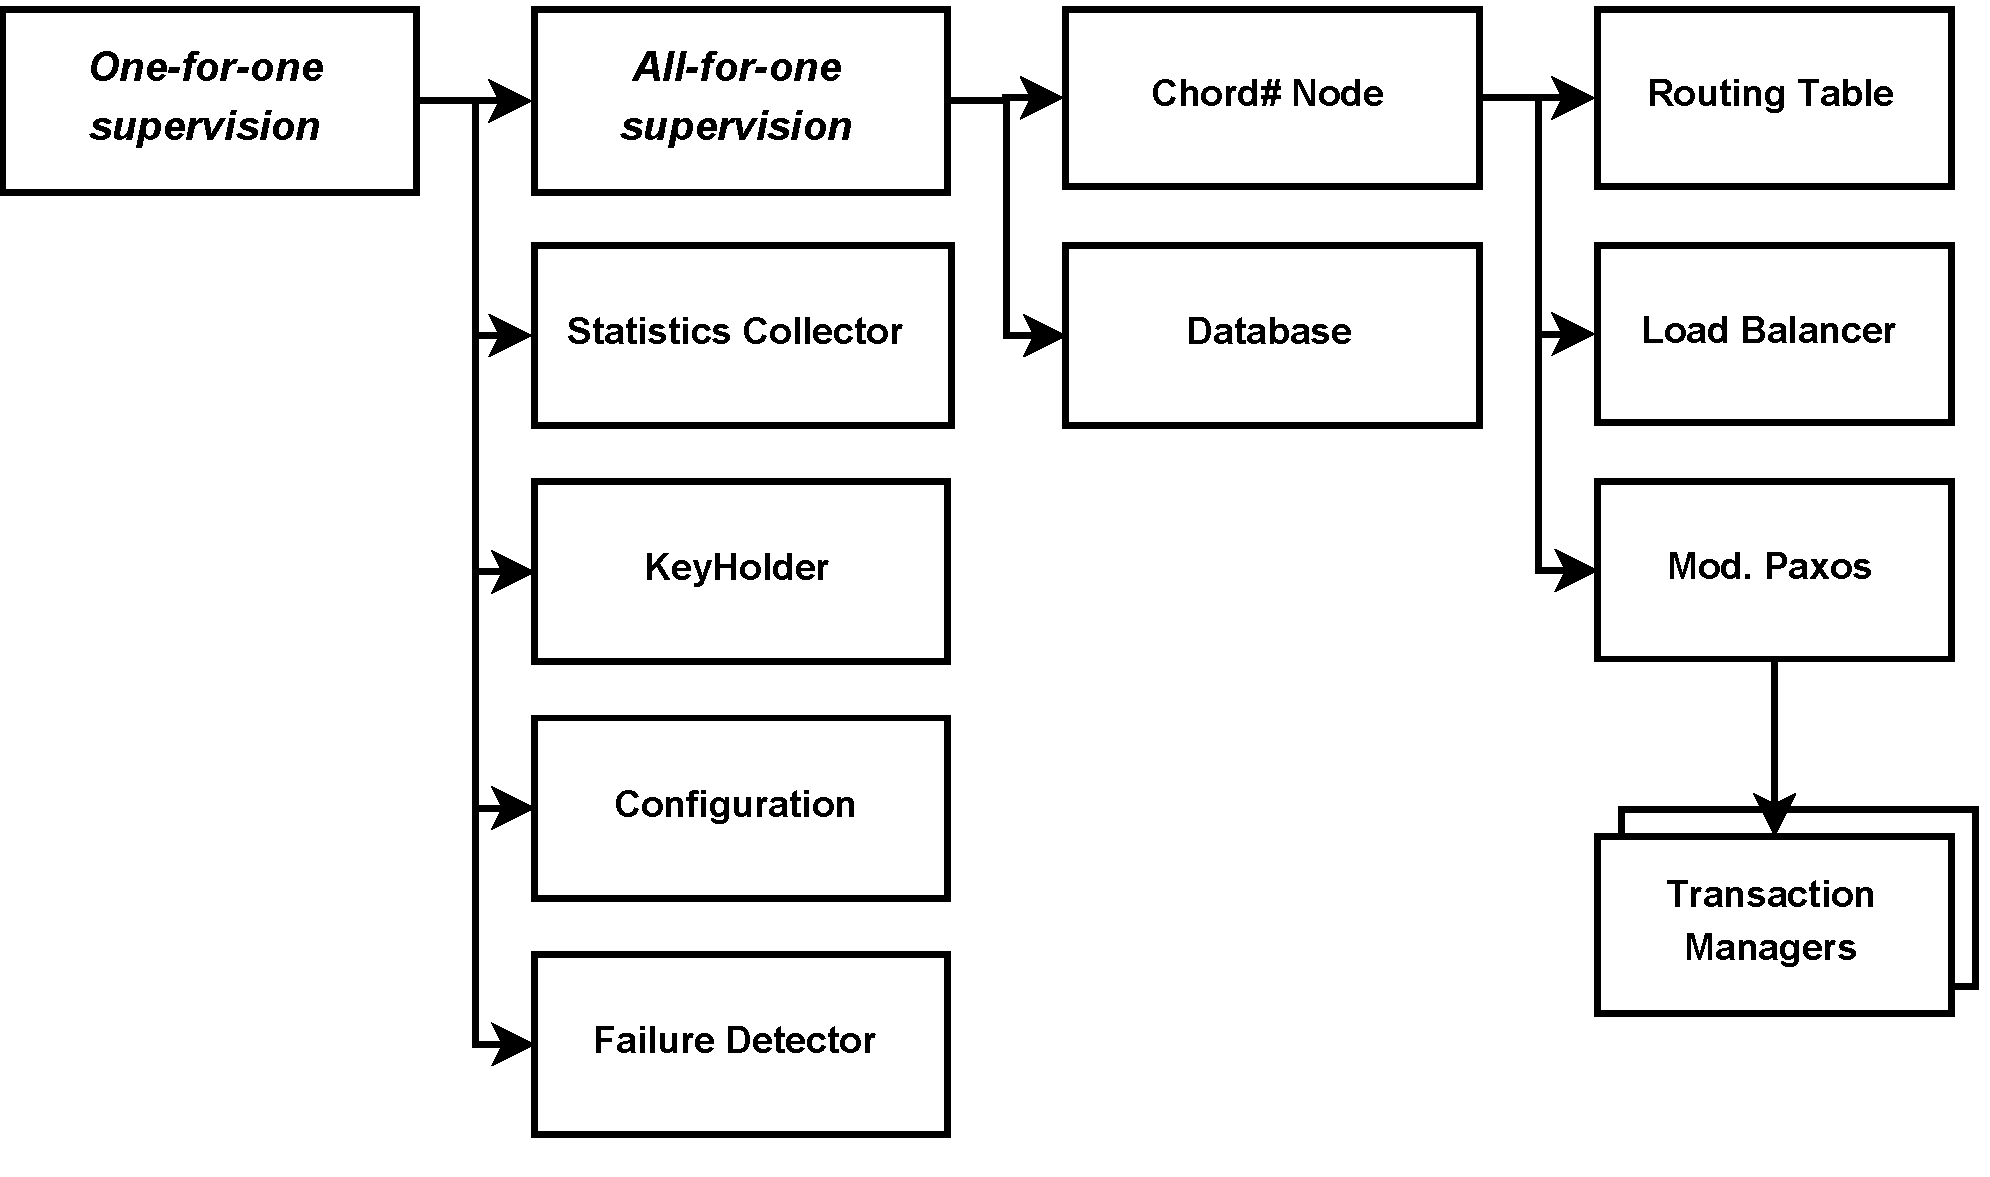
\includegraphics[width=0.9\linewidth]{supervision}}

\subsection{Starting the or-supervisor and general processes of a node}

Starting supervisors is a two step process: the supervisor mechanism
first calls the \code{init()} function of the defined module
(\code{sup_dht_node:init()} in this case) and then calls the start
function (\code{start_link} here.

So, lets have a look at \code{sup_dht_node:init}, the 'Scalaris
\emph{or} supervisor'.

\codesnippet{sup_dht_node.erl}{sup_dht_node:init}{../src/sup_dht_node.erl}


The return value of the \code{init()} function specifies the child
processes of the supervisor and how to start them. Here, we define a
list of processes to be observed by a \code{one_for_one}
supervisor. The processes are: \code{KeyHolder}, \code{DeadNodeCache},
\code{RingMaintenance}, \code{RoutingTable}, and a
\code{Supervisor_AND} process.

The term \code{\{one_for_one, 10, 1\}} specifies that the supervisor
should try 10 times to restart each process before giving
up. \code{one_for_one} supervision means, that if a single process
stops, only that process is restarted. The other processes run
independently.

The \erlfun{sup\_dht\_node}{init}{} is finished and the supervisor module,
starts all the defined processes by calling the functions that were
defined in the list of the \erlfun{sup\_dht\_node}{init}{}.

For a join of a new node, we are only interested in the starting of
the \code{Supervisor_AND} process here. At that point in time, all
other defined processes are already started and running.

\subsection{Starting the and-supervisor with a peer and its local database}

Again, the OTP will first call the \code{init()} function of the
corresponding module:

\codesnippet{sup_dht_node_core.erl}{sup_dht_node_core:init}{../src/sup_dht_node_core.erl}

It defines three processes, that have to be observed using an
\code{one_for_all}-supervisor, which means, that if one fails, all have to
be restarted. Passed to the \code{init} function is the \code{InstanceId}, a
random number to make nodes unique. It was calculated a bit earlier in
the code. Exercise: Try to find where.

As you can see from the list, the \code{DB} is started before the
\code{Node}. This is intended and important, because \code{dht_node} uses
the database, but not vice versa. The supervisor first completely
initializes the DB process and afterwards calls
\erlfun{dht\_node}{start\_link}{}. We only go into details here, for the
latter.

\codesnippet{dht_node.erl}{dht_node:start_link}{../src/dht_node.erl}

\erlmodule{dht\_node} implements the \code{gen_component} behaviour. This
component was developed by us to enable us to write code which is
similar in syntax and semantics to the examples in~\cite{rachid-book}.
Similar to the \code{supervisor} behaviour, the component has to
provide an \code{init} function, but here it is used to initialize the
state of the component. This function is described in the next
section.

Note: \code{?MODULE} is a predefined Erlang macro, which expands to the
module name, the code belongs to (here: \code{dht_node}).

\subsection{Initializing a \code{dht_node}-process}

\codesnippet{dht_node.erl}{dht_node:start}{../src/dht_node.erl}

The \code{gen_component} behaviour registers the \code{dht_node} in the
process dictionary. Formerly, the process had to do this himself, but
we moved this code into the behaviour. If the \code{dht_node} is the
first node, he will start immediately. Otherwise, the process sleeps
for a random amount of time. If you would start 1000 processes with
\erlfun{admin}{add\_nodes}{1000}, the boot-server would receive many join
requests at the same time, which is not intended. It will also make
the ring stabilization process more complicated. Adding 100s of nodes
within a short period of time induces more churn into the system, than
the ring maintenance can handle.

Then, the node retrieves its \code{Id} from the keyholder: \code{Id =
  cs_keyholder:get_key()}. In the first call, a random identifier is
returned, otherwise the latest set value. If the \code{dht_node}-process
failed and is restarted by its supervisor, this call to the keyholder
ensures, that the node still keeps its \code{Id}, assuming that the
keyholder process is not failing.  This is important for the load-balancing
and for consistent responsibility of nodes to ensure consistent lookup in
the structured overlay. Note: the name \code{Key-holder} actually is an
id-holder.

If a node changes its position in the ring for load-balancing, the
key-holder will be informed and the \code{dht_node} finishes itself. This
triggers a restart of the corresponding database process via the
and-supervisor.  When the supervisor restarts both processes, they will
retrieve the new position in the ring from the key-holder and join the ring
there.

\todo{The supervisor was configured to restart a node at most 10 times. Does
  that mean, that a node can only change its position in the ring 10 times
  (caused by load-balancing)?}

%Next, the \code{dht_node} registers itself as the owner of the
%failuredetector \code{failuredetector:set_owner(self())} to become informed,
%when the failuredetector detects failing nodes.

%With \code{boot_server:connect()} a connection to the boot-server is
%established.

\subsection{Actually joining the ring}

After retrieving its identifier, the node starts the join process
(\erlfun{dht\_node\_join}{join}{}).

\codesnippet{dht_node_join.erl}{dht_node_join:join1}{../src/dht_node_join.erl}

The boot-server is contacted to retrieve the known number of nodes in the
ring. If the ring is empty, \code{join_first} is called. Otherwise,
\code{join_ring} is called.

If the ring is empty, the joining node is the only node in the ring
and will be responsible for the whole key space. \code{join_first}
just creates a new state for a \scalaris{} node consisting of an empty
routing table, a successorlist containing itself, itself as its
predecessor, a reference to itself, its responsibility area from
\code{Id} to \code{Id} (the full ring), and a load balancing schema.

\codesnippet{dht_node_join.erl}{dht_node_join:join_first}{../src/dht_node_join.erl}

The macro \code{?RT} maps to the configured routing algorithm and
\code{?RM} to the configured ring maintenance algorithm. It is defined
in \code{include/scalaris.hrl}. For further details on the routing see
Chapter~\sieheref{chapter.routing}.

The state is defined in

\codesnippet{dht_node_state.erl}{dht_node_state:state}{../src/dht_node_state.erl}

If a node joins an existing ring, \code{reliable_get_node} is called for the
own \code{Id} in \erlfun{dht\_node\_join}{join}{}. This lookup delivers the
node who is currently responsible for the new node's identifier -- the
successor for the joining node. If this lookup fails for some reason, it is
tried again, by recursively calling the \code{join()}.

\todo{What, if the \code{Id} is exactly the same as that of the existing
  node? This could lead to lookup and responsibility inconsistency? Can this
  be triggered by the load-balancing? This is a bug, that should be
  fixed!!!}

Then, \erlfun{dht\_node\_join}{join\_ring}{} is called:

\codesnippet{dht_node_join.erl}{dht_node_join:join_ring}{../src/dht_node_join.erl}

First the node is initialized. Then it sends a \code{join} message to the
successor including a reference to itself and the chosen \code{Id}.

The message is received by the old node in \code{dht_node.erl}. There exists
a \code{\{join, X\}} handler.

\codesnippet{dht_node.erl}{dht_node:join_message}{../src/dht_node.erl}

This triggers a call to \code{join_request} on the old node.

\codesnippet{dht_node_join.erl}{dht_node_join:join_request}{../src/dht_node_join.erl}

The \code{dht_node} notifies the ring maintenance, that he has a new
predecessor. Then he removes the key-value pairs from his database
which are now in the responsibility of the joining node. Then it
sends a \code{join_response} to the new node with its former
predecessor, the data, it has to host, and its successorlist.

%Note: Here, the observation of the former predecessor could be deleted from
%the failure detector. But periodically, all known hosts are reregistered
%with the failure detector, and then all other nodes are thrown away from the
%list of nodes to observe in the failure detector. So, we do not care here.

%Finally, the new predecessor is set and the \code{join_request()} is finished.


Back on the joining node: it waits for the \code{join_response}
message in \erlfun{dht\_node\_join}{join\_ring}{}. The next steps after the
message was received from the old node are to initialize the
maintenance components for the ring and routing table, the database
and the state of the \code{dht_node}.

\subsection{Beginning to serve requests}

\erlfun{dht\_node\_join}{join}{} was called from \erlfun{dht\_node}{start}{},
which now continues

\codesnippet{dht_node.erl}{dht_node:start}{../src/dht_node.erl}

The \erlfun{cs\_replica\_stabilization}{recreate\_replicas}{} function is
called, which is not yet implemented. It would recreated necessary replicas
that were lost due to load-balancing and node failures.

Finally, the loop for request handling is started.

% \subsection{FAQ}

% \paragraph{Question:} How are the routing-table, load-balancing and paxos 
%   processes started, that can be seen in the supervisor tree?

%   \paragraph{Answer:} They are currently not implemented as separate Erlang
%   processes. All the requests are handled by the loop started by
%   \code{dht_node:start()}. Nevertheless, they could be implemented as
%   separate processes to make the software architecture cleaner.

\chapter{Directory Structure of the Source Code}

The directory tree of \scalaris{} is structured as follows: \\

\begin{tabular}{|r|p{11.5cm}|}
 \hline
 \code{bin} & contains shell scripts needed to work with \scalaris{} (e.g.\ start the boot services, start a node, \dots)\\
 \code{contrib} & necessary third party packages (yaws and log4erl) \\
 \code{doc} & generated erlang documentation \\
 \code{docroot} & root directory of the bootserver's webserver \\
 \code{docroot_node} & root directory of the normal node's webserver \\
 \code{ebin} & the compiled Erlang code (beam files)\\
 \code{java-api} & a java api to \scalaris{} \\
 \code{log} & log files \\
 \code{src} & contains the \scalaris{} source code\\
 \code{test} & unit tests for \scalaris{} \\
 \code{user-dev-guide} & contains the sources for this document\\
 \hline
\end{tabular}

%\chapter{System Components}



%\chapter{Processes}

%\chapter{Troubleshooting}

%\section{ApplicationMonitor appmon:start()}

\chapter{Java API}

For the Java API documentation, we refer the reader to Javadoc
resp. doxygen. The following commands create the documentation:

\begin{lstlisting}[language=sh]
%> cd java-api
%> ant doc
%> doxygen
\end{lstlisting}

The Javadoc can be found in \code{java-api/doc/index.html}. The
doxygen is in \\ \code{doc-doxygen/html/index.html}.

We provide two kinds of APIs:

\begin{itemize}
\item high-level access with \code{de.zib.scalaris.Scalaris}
\item low-level access with \code{de.zib.scalaris.Transaction}
\end{itemize}

The former provides general functions for reading and writing single
key-value pairs and an API for the built-in PubSub-service. The latter
allows the user to write custom transactions which can modify an
arbitrary number of key-value pairs within one transaction.

\bibliographystyle{plainnat}

\begin{thebibliography}{9}

\bibitem{erlang-book}
Joe Armstrong.
\newblock \emph{Programming Erlang: Software for a Concurrent World.}
\newblock Pragmatic Programmers, ISBN: 978-1-9343560-0-5, July 2007

\bibitem{rachid-book}
Rachid Guerraoui and Luis Rodrigues.
\newblock \emph{Introduction to Reliable Distributed Programming.}
\newblock Springer-Verlag, 2006.

\end{thebibliography}

\printindex

\end{document}
%%% Local Variables: 
%%% mode: latex
%%% TeX-master: t
%%% End: 

